%!TEX root = ../main.tex

%
% Notes: 
%
%  exact implementation
%  comparison with rollback at batch N
%  relaxing the solvers
%  dealing with false positives
%
%  running on TPC-C/sanjay's.  equality is easier
%
% Need names for
%  * rollback
%  * exact solution
%  * fixing an individual/batch of queries
%
\section{Experiments}

In this paper, we have described several heuristic algorithms based on decision trees 
and bounding box algorithms \alex{do we talk about bounding box algorithms?}, as well as an exact, albeit less-scalable,
constraint-based solution to the \prob problem.  In addition, we 
introduced  several extensions to the MILP-based solution~\alex{We should be careful and not tie it to CPLEX.  CPLEX is just a particular solver.  ILP-based is better.} that 
1) improves the scalability of the system and 2) tolerates false positives and 
negatives in the input complaint set.
\alex{The wording is a bit anemic.  It makes it sound like we suggested a few naive approaches and hacks.  Add more oomph!}
Our goals in the evaluation is to understand these trade-offs in
controlled synthetic scenarios, as well as study the effectiveness
in typical database query workloads based on widely used benchmarks.

To this end, our experiments are organized as follows: First, 
we compare the exhaustive MILP algorithm against the different optimizations 
to highlight the value of different optimizations.  We then compare the
repair costs of \texttt{INSERT}, \texttt{DELETE}, or \texttt{UPDATE}-only query logs 
and find that the latter query type is by far the most complicated and costly to repair.
For the subsequent experiments, we focus solely on \texttt{UPDATE}-only synthetic workloads 
to understand how \sys responds to different query logs and databases.  
Finally, we evaluate the efficacy on real-world databases transaction benchmarks,
TPC-C XXX~\cite{tpcc} and AuctionMark~\cite{auctionmark}.



% establish the quality limitations of existing heuristics and the need for a formal, 
% constraint-based algorithm (\exact).  Second, we study how each of the 
% optimizations described in Section~\ref{s:optimiztaions} improves algorithm scalability.
% Third, we introduce different forms of error in the input complaint sets and study the 
% effectiveness of our noise-handling heuristics.  




%
% NOTE: figures are named <experimentsection>_<subsection>_<xaxis>.pdf
%

\subsection{Experimental Setup}


\begin{table}[t]\small
  \centering
  \begin{tabular}{@{}cll@{}}
  \toprule
  {\bf Param} & {\bf Description} & {\bf Default} \\ \midrule
  $V_d$  & Domain range of the attributes  & $[0, 100]$ \\
  $N_D$  & \# tuples in final database & $1000$ \\
  $N_a$  & \# attributes in database & $10$ \\
  $N_w$  & \# predicates in \texttt{WHERE} clauses & $1$ \\
  $N_s$  & \# \texttt{SET} clauses & $1$ \\
  $N_q$  & \# queries in query log & $300$ \\
  $idx$  & Index (backwards from most recent) & $\{0, 25, 50,$ \\
         & of corrupted query & $100, 200, 250 \}$ \\ %$\frac{N_q}{2}$ \\
  $r$    & Range size of \texttt{UPDATE} queries & 8 (tuples) \\
  $s$    & Zipf $\alpha$ param of query attributes, & $1$ \\ 
  $set$  & Constant vs relative \texttt{SET} clauses. & const \\ \bottomrule \end{tabular}
         %& power low distribution $P(v) = v^{-s}$ & \\\end{tabular}
  \caption{Experimental Parameters \alex{Do we need the presentation to include this level of detail?}}
  \label{t:params}
\end{table}


\begin{table}[t]\small
  \centering
  \begin{tabular}{@{}cl@{}}
  \toprule
  {\bf Param} & {\bf Description} \\ \midrule
  $p$ & Precision: \% of repaired tuples that are correct. \\
  $r$ & Recall: \% of full complaint set repaired.\\
  % $t_{prep}$ & Time to construct CPLEX problem \\
  % $t_{send}$ & Time to send CPLEX problem to solver \\
  % $t_{solve}$ & Time for solver to generate a solutions\\
  $t_{total}$ & End-to-end execution time \\ 
  $d_{measure}$ & \red{Some sort of distance measure} \\ \bottomrule \end{tabular}
  \caption{Metrics Compared}
  \label{t:metrics}
\end{table}



\ewu{one point to know is that the recall can only be less than 1 in two cases:
1) incomplete complaint set 2) Solver infeasibility.  If the complaint set
is complete and the solver returns a solution, the recall will be $1$. 
This point is important to emphasize.}

Each of our experiments follows a consistent procedure. 
We generate a sequence of queries using a synthetic query generator or 
the benchmark program, and corrupt the query log as described below. 
We then execute the original and corrupt query logs on an initial (possibly empty) database,
and perform a tuple-wise comparison between the resulting database states 
to generate a true complaint set.  
We then add noise to the complaint set by 1) picking random tuples not in the true
complaint set to add false positive complaints, and 2) removing true complaints to simulate false negatives.
Finally, we execute the evaluated algorithms on the complaints and compare the fixed
query log with the true query log, as well as the fixed and true
final database states to measure performance and accuracy metrics.

We compare the following algorithms:
$\sys_{exh}$ the naive, exhaustive MILP algorithm; 
$\sys_{S \subseteq \{t,q,a,inc\}}$ where the subscripts $t,q,a,inc$ represent the
application of tuple, query and attribute slicing and incremental computation -- 
for example, $\sys_{t,q,inc}$ uses both tuple and query slicing along with the incremental computation; 
when the algorithm uses incremental computation, the superscripts $\sys_{inc}^{first}$
and $\sys_{inc}^{all}$ describe the incremental algorithm that either returns the first successful repair,
or returns the repair with the lowest objective function across the entire query log.

We evaluate the algorithms along several metrics.  Performance is measured as wall clock
time between submitting a query log and retrieving the results.  In Experiment~\ref{???},
we evaluate the total time to output {\it each repair} when running the incremental algorithm
across the entire query log.  In addition, we measure the repair's precision (percentage of
repaired tuples that were correctly fixed), the recall (the percentage of the full complaint set that was 
repaired), and the F1 measure (the harmonic mean of precision and recall).
Table~\ref{t:params} summarizes the key parameters that we vary throughout our experiments.  
The rest of this section outlines our datasets, workloads, and parameters used to generate the data 
and query logs in our experiments.

{
\color{blue} 
We ran experiments on machines with 
2.66 GHz processor and 16GB RAM. 
}
\alex{Why is this description separate from the synthetic data listed below?}

\subsubsection{Datasets and Workloads}

This subsection describes the query and data generation process in greater detail.

\stitle{Synthetic} \label{sec:syntheticgen}
{\color{blue} We generate an initial database of $N_D$ random tuples.  
The schema contains $N_a=5$ attributes $a_1\ldots a_5$, whose values are
picked from $V_d$ uniformly at random, along with a primary key $id$.
We then generate a sequence of $N_q$ \texttt{UPDATE} queries, which
have the following respective forms: where \verb|?| is a query parameter 
and \verb|r| is the size of the range. }
\iffalse
  We generate an initial database of $N_D$ random tuples.  
  The schema contains $N_a=5$ attributes $a_1\ldots a_5$, whose values are
  picked from $V_d$ uniformly at random, along with a primary key $id$.
  We then generate a sequence of $N_q$ queries containing a mixture of \texttt{INSERT} queries,
  point \texttt{UPDATE} queries, and range \texttt{UPDATE} queries.  
  The \texttt{UPDATE} queries have the following respective forms, where \verb|?| is a query parameter 
  and \verb|r| is the size of the range.
\fi
{\scriptsize
\begin{verbatim}
  UPDATE SET (a_i = ?),.. WHERE a_j = ? AND ...
  UPDATE SET (a_i = ?),.. WHERE a_j in [?, ?+r] AND ...
\end{verbatim}
}

The $set$ parameter controls whether the \texttt{UPDATE} queries set attributes to random constant values ({\it const}),  
or increment attributes by a random amount ({\it rel}).  The \texttt{WHERE} clauses form a conjunction.
In addition we varied a skew parameter $s$, which determines the attributes referenced in the \texttt{WHERE}
and \texttt{SET} clauses.  Each attribute in a query is picked from either a uniform distribution or 
a zipfian~\cite{zipf} distribution
with exponent $0+s$.  This allows our experiments to vary between a uniform distribution, where each attribute is
equally likely to be picked, and a skewed distribution where nearly all attributes are the same. \\
\iffalse
  \texttt{INSERT} queries simply insert values picked uniformly at random from $V_d$.  

  \xlw{Replace with what we actually do:
  We first consider three different homogenous query logs: \texttt{INSERT} only ($p_I = 1$), 
  \texttt{PK} update only ($p_I = 0, p_{pk} = 1$), and \texttt{RANGE} update only ($p_I = 0, p_{pk} = 0$).
  These query logs help us understand \sys's performance characteristics for each query type individually.  
  Finally, we investigate heterogenous mixtures of the three query types to simulate varying amounts of real settings.
  } \\
  \xlw{We only have UPDATE query in the synthetic dataset. In single error case, how to fix a insert query is 
  quite straightforward as well as the delete query. Should we cut words for insert and delete query?}
\fi


% \begin{figure}[h]
% \centering
% 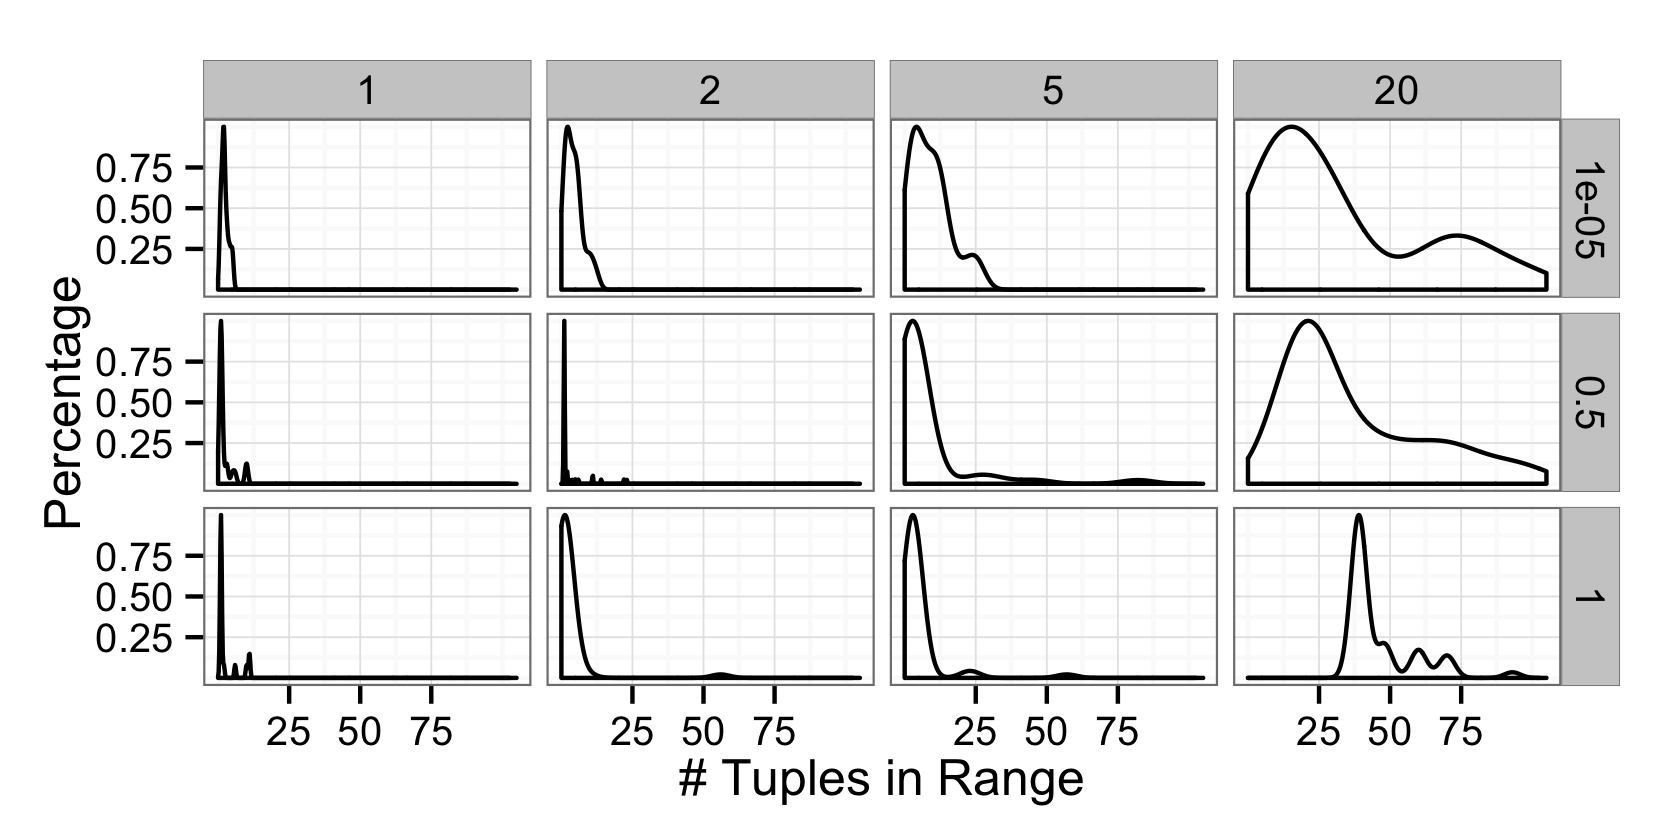
\includegraphics[width = 3.5in]{figures/qidxsimulation/numinrange}
% \caption{.}
% \label{f:numinrange} 
% \end{figure}



% Anant's workload?
{ \color{blue}
\stitle{TPC-C} We use the data and query workload over the {\it
ORDER} table in TPC-C~\cite{}.  We generate a database at scale
1 with one warehouse, and keep only the queries that modify the
{\it ORDER} table. The initial table contains 4570 tuples and we capture 
1000 queries in which 530 are \texttt{UPDATE} query and the others
are \texttt{INSERT} query. 
%We then randomly perturb a subset of the queries to generate the corrupted query log. 
We pick query at certain index ($idx$ in Table~\ref{t:params}) 
and corrupt it by replacing the correct parameter(s) into randomly 
generated incorrect one(s) according to the corresponding attribute domain. 

\stitle{AuctionMark} Auctionmark workload simulates the 
actual action market. We generate a database 
with 8729 tuples and 650 queries (540 \texttt{UPDATE} query and 110 \texttt{INSERT} query) 
and we perturb the query log in the same way as for the TPC-C workload.

Both workloads generated from the OLTP-bench project~\cite{oltpbench,oltpbenchgit}.



}
{\color{blue}
\subsection{Single-Query Comparison}
In this section, we compare \heurstic and \milpall on query log with size 1. 
We use \textbf{Synthetic} data generator (Section~\ref{sec:syntheticgen}) 
to generate a initial table with 1000 tuples and one 
\texttt{UPDATE} query with range update. 
We further adjust the range (\# of tuples modified by the query) 
from 5 tuples to 500 tuples. 

 \begin{figure}[h]
\centering
  \begin{subfigure}[t]{.48\columnwidth}
  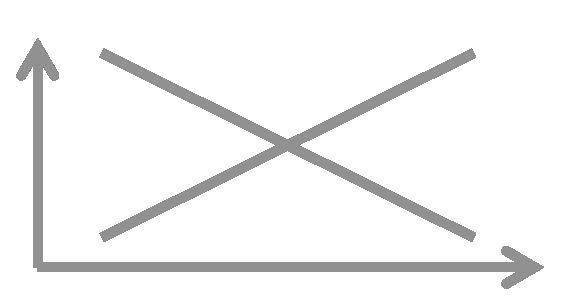
\includegraphics[width = .95\columnwidth]{figures/placeholder}
  \caption{.}
  \label{f:heursticvsmilp} 
  \end{subfigure}
  \caption{Heuristic Approach vs. MILP-based Approach on Single-Query. }
\end{figure}

\subsection{Multi-Query Comparison}
We further compare \milpall, \milptuple, \milptuplestopearly, \milpadvtuple  
on \textbf{Synthetic} data 
with 1000 tuples and 300 queries. We adjust the problem complexity by corrupting queries 
at different indexes: as we error happen further from the most recent query, 
the problem become harder to solve. 

\begin{figure}[h]
\centering
  \begin{subfigure}[t]{.48\columnwidth}
  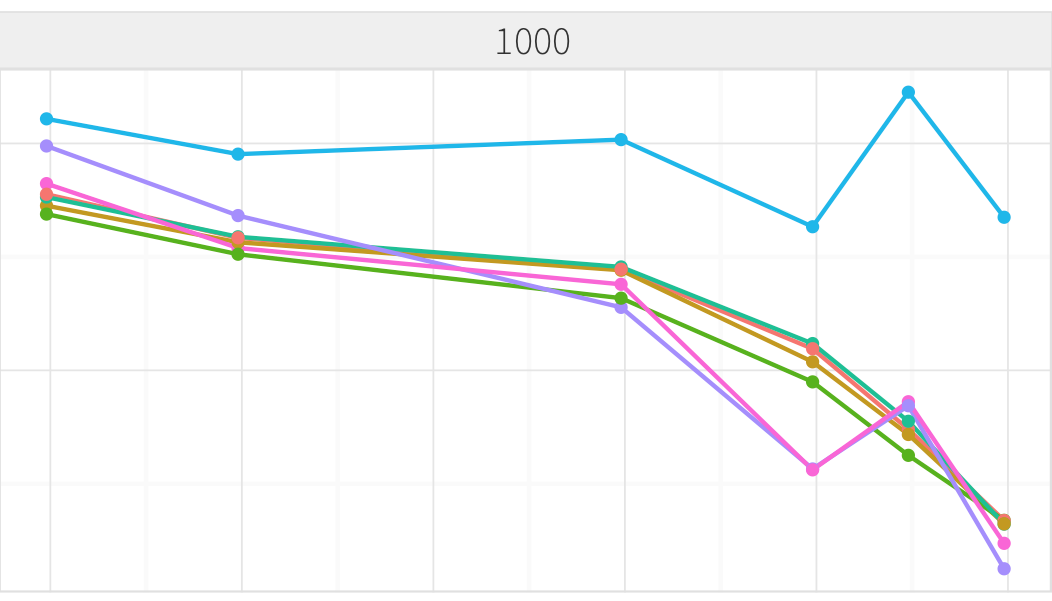
\includegraphics[width = .95\columnwidth]{figures/scale_allalgs}
  \caption{.}
  \label{f:multiquery} 
  \end{subfigure}
  \caption{MILP-based Approach and Extensions on Multi-Query. }
\end{figure}



\subsubsection{Updates Matter}
Run insert and delete only workloads.
Show that update queies are the really hard ones



\subsubsection{Comparing Optimization Options}

EXP 1
Compare all algorithms for a varying number of corrupted queries.
% - exh, tupleslice, queryslicing, attrslicing, tuplequeryslicing
% - 1 error: oldest query
% - 2 errors: oldest query + 10th
% - 3 errors: oldest + 10th + 20th
% - dbsize: 1000
% - uniform skew
Show that exhaustive and exh+t,q,a are all incredibly slow and the optimizations help a bit.

EXP 2
Compare exh+optimizations, inc and shows that inc is way better.

End up picking $queryfix_{inc,t}$, $queryfix_{inc,t,q}$
Justify single corrupt query

\subsubsection{Synthetic Experiments}

\subsubsection{Noise}

\subsubsection{Benchmarks}

\subsubsection{Incremental Results}

INcremental algorithm, incremental results


%
% compair everything, naive sucks
% 
% add compare everything with multiple corrupted queries
% - exh, tupleslice, queryslicing, attrslicing, tuplequeryslicing
% - 1 error: oldest query
% - 2 errors: oldest query + 10th
% - 3 errors: oldest + 10th + 20th
% - dbsize: 1000
% - uniform skew
% 
% zoom in onto: inc, inc+tupleslicing, inc+query slicing, inc+attrslicing, everything (cplex2)
% 
% pick cplex2 as the winner
% 
% cplex_searchall = incremental but for everything
% 
% cplex3 == cplex_stop_early_2iter
% 
% the naive algorithms suck.
% 
% incremental comptuation vs non incremental comptutaion
% 
% show that w/wout query fix is what makes the difference
% incremental should always be on



\noindent {\it Effect of Index of Corrupted Query:}
A key parameter for our experiments is the location of the corrupted query ($idx$).  
\alex{Have we discussed anywhere yet that we focus on single errors?}
This parameter determines the number of queries \sys must consider when searching for a fix,
and affects the size of the complaint set.  
\alex{It won't be clear to the reader how this relates to the size of the complaint set.}
Both of these characteristics directly impact \sys's 
runtime performance. For this reason, it is undesirable to randomly pick and corrupt queries
throughout the query log, as the performance and accuracy results may not be comparable. 
To better understand the relationship between $idx$ and the size of the complaint set, we ran
simulations using a database with $20$ attributes, and a query log of size $1000$ containing
either all $set = const$ or $set = rel$ \texttt{UPDATE} queries.
We varied  $idx$ uniformly throughout the query log, and additionally varied
the skew $s$ and range $r$ parameters to study how they affect the size of the complaint sets.


  \begin{figure}[h]
  \centering
  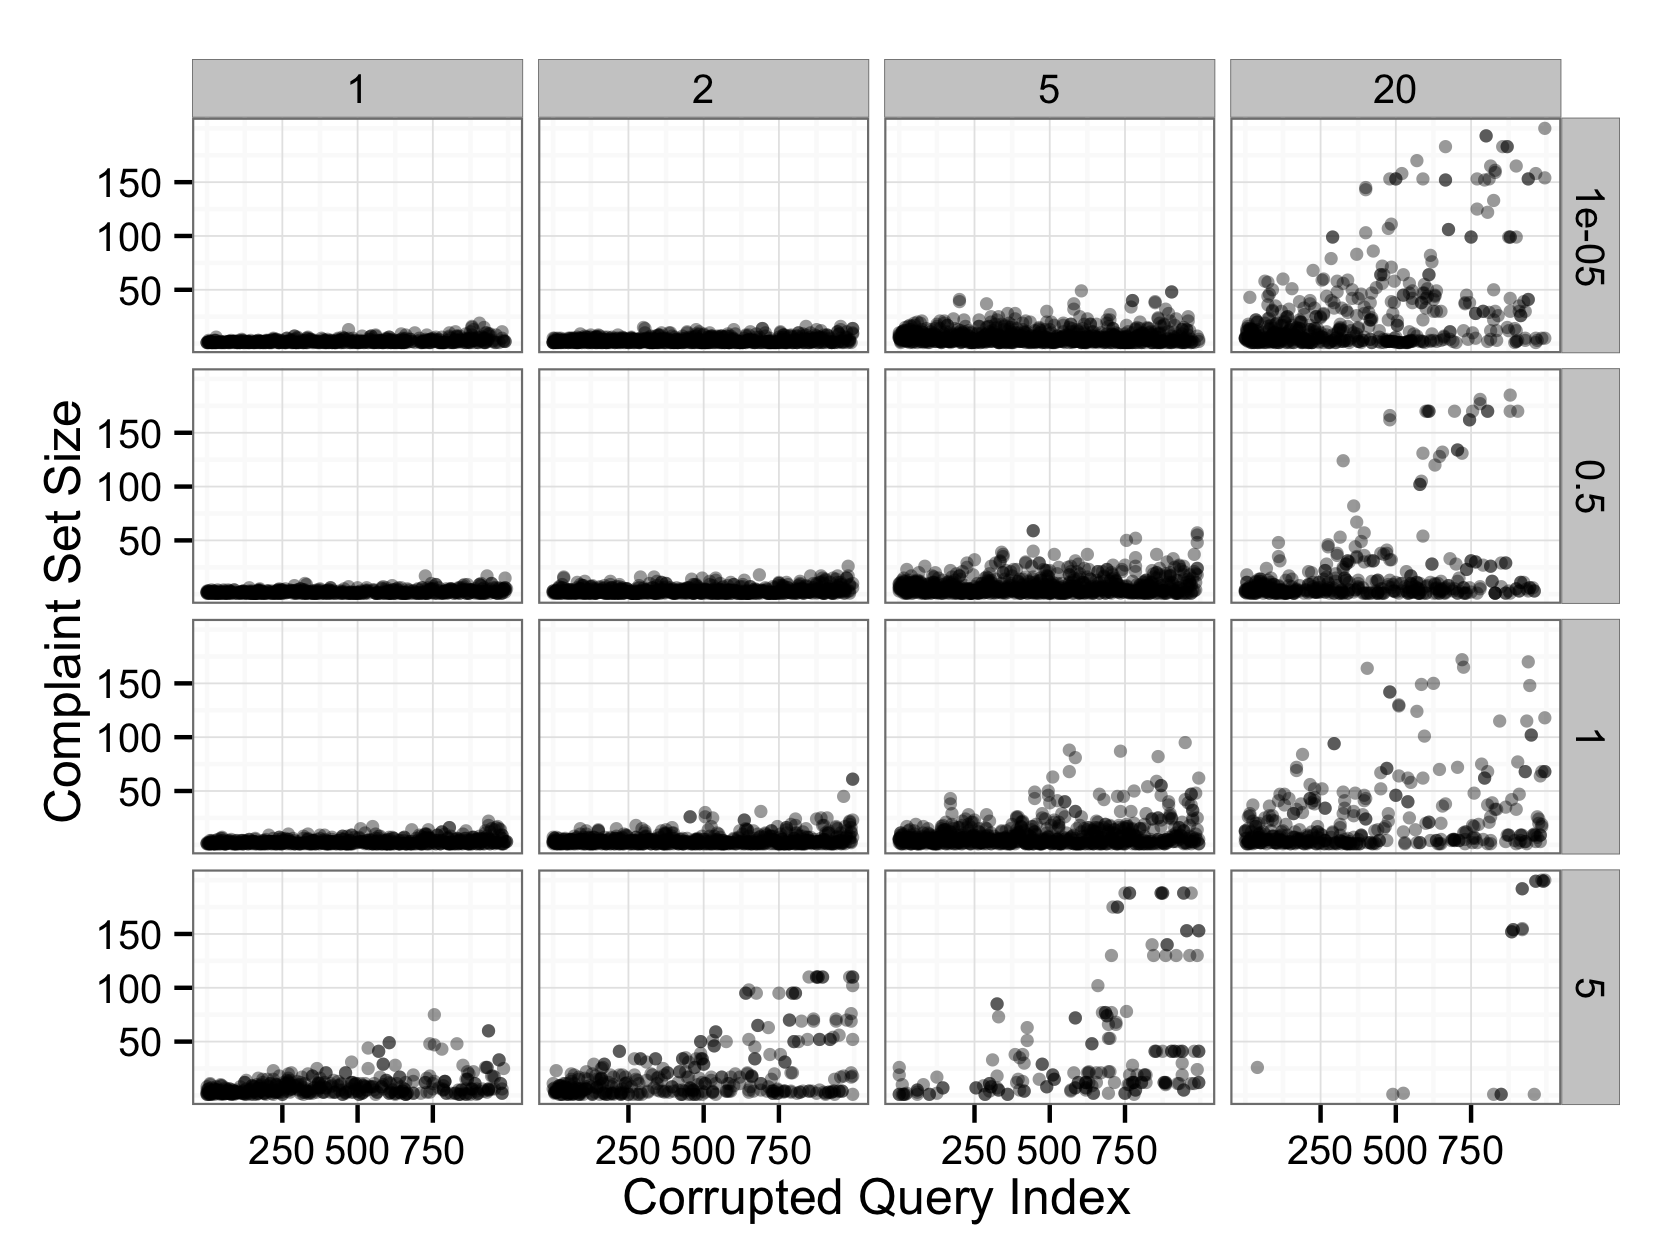
\includegraphics[width = 3.5in]{figures/qidxsimulation/qidx_v_ncomplaints_20attrs_const}
  \caption{Query index vs complaint set size for $set = const$.}
  \label{f:qidx_v_ncomplaints_const} 
  \end{figure}


Figure~\ref{f:qidx_v_ncomplaints_const} plots a representative set of parameters.  We plot one point
for each corrupted query index that results in a complaint set with at least one complaint. 
These results highlight several interesting trends.  When queries do not overlap ($r = 1$, leftmost column),
the size of the complaint sets are relatively small, and their frequency is constant across the possible query indices.
However as the possibility of overlap increases (e.g., $r$ increases), more recent queries are more likely to result in
very large complaint sets (at times the size of the database).   
This effect is a symptom of the fact that queries with large ranges will set groups of tuples to the same value,
and over time, skew the distribution of tuple values to a small number of possible values.
Thus, more recent corruptions that affect a large cluster of similar tuples will result in a large complaint set.
We find that increasing the skew parameter also exacerbates this effect.  
In addition, high skew increases the likelihood that queries will share the same \texttt{WHERE} and \texttt{SET} clause 
attributes as a corrupted query, thus overwriting the error introduced by the corrupted query.  
This is why the frequency of non-empty complaint sets decreases significantly as $s$ increases.


\begin{figure}[h]
\centering
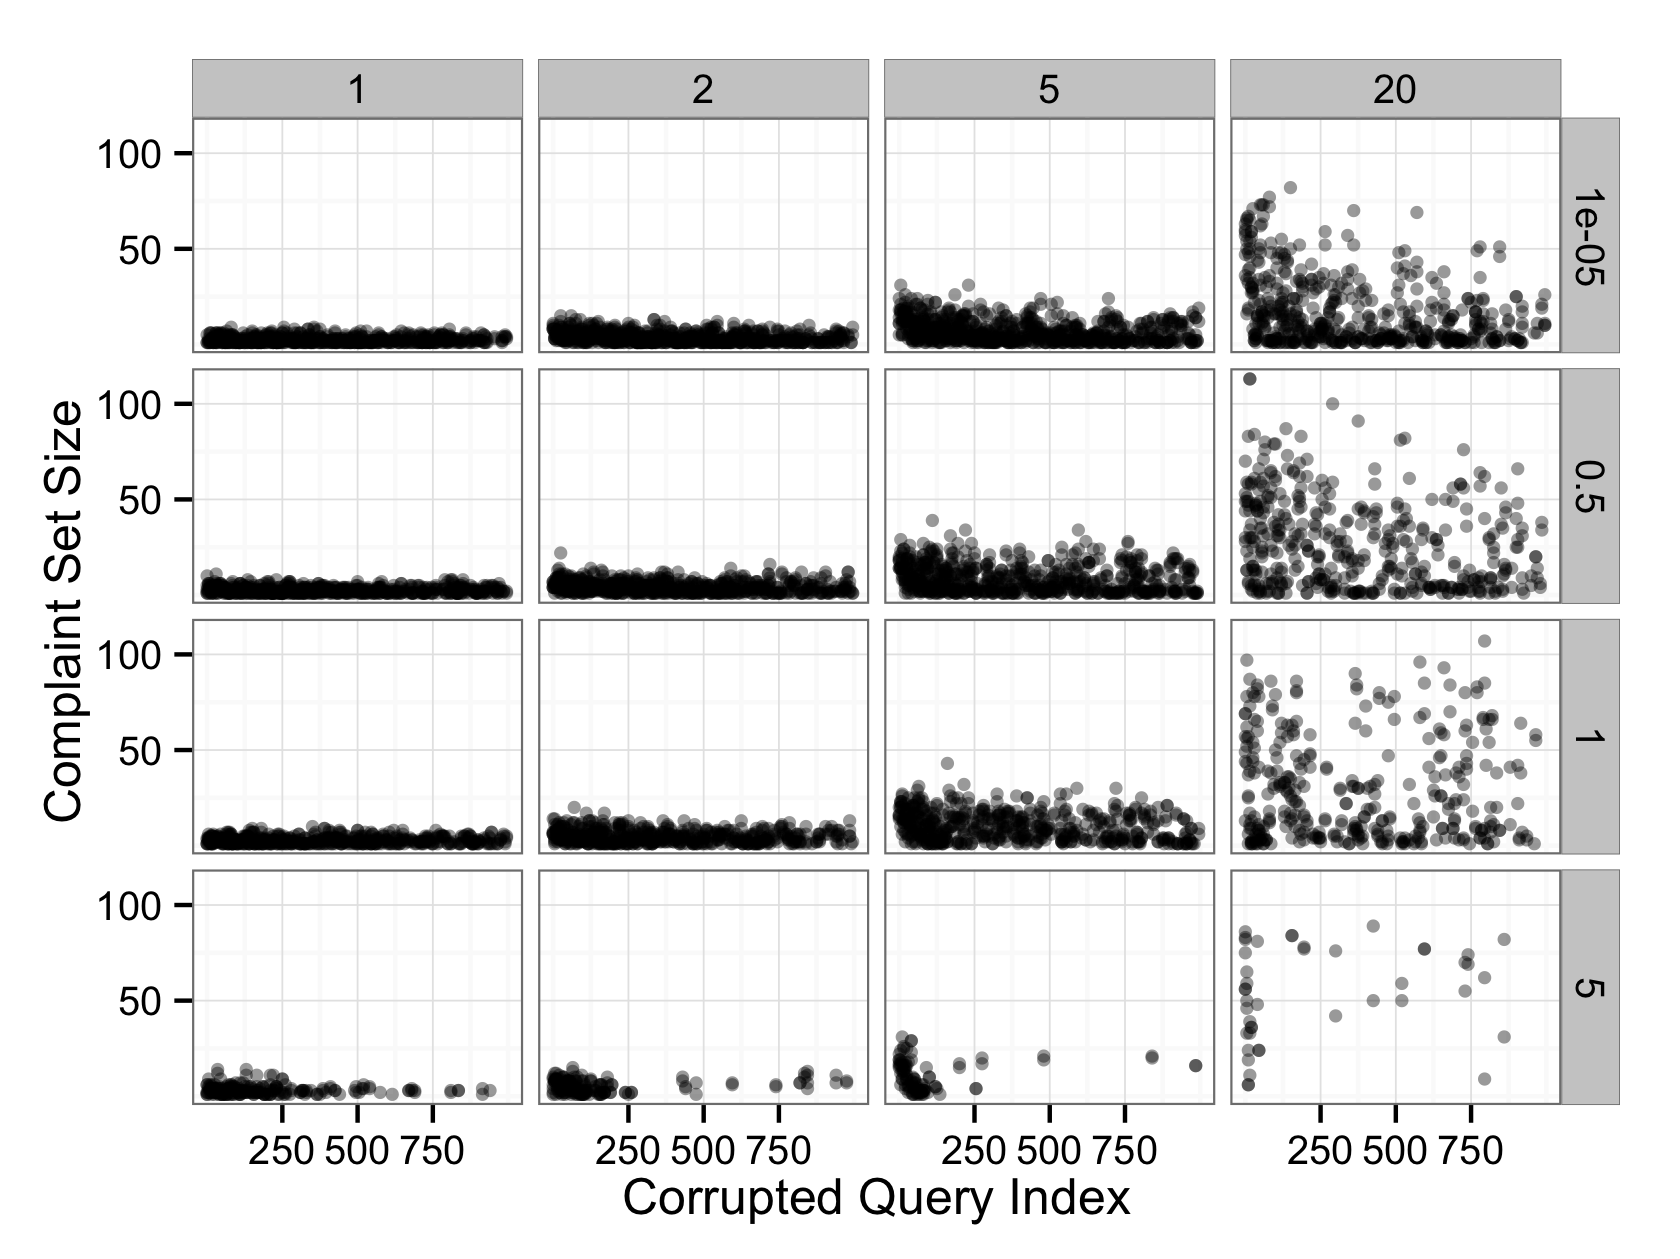
\includegraphics[width = 3.5in]{figures/qidxsimulation/qidx_v_ncomplaints_20attrs_rel}
\caption{Query index vs complaint set size for $set = rel$.}
\label{f:qidx_v_ncomplaints_rel} 
\end{figure}

In contrast to $set=const$ queries, Figure~\ref{f:qidx_v_ncomplaints_rel} executes the 
same experiment using $set=rel$ queries.  In this setting, we find that the trend is
reversed, and older corruptions tend to result in larger complaint sets.  This is because,
subsequent \texttt{UPDATE} queries increment or decrement the attribute value, rather than
overwriting it with a constant value.  The clustering of data values due to query overlap
then increases the number of other tuples affected.


\ewu{summarize findings and implications to experiments here.}
not all corruptions result in complaint sets.
In constant SET clause workloads, larger complaints sets are more likely to
result from more recent corrupted queries -- particularly if the queries are range updates or
the updated attributes are skewed.
For this reason, our experiments corrupt the query log at six positions 
$idx \in \{0, 25, 50, 100, 200, 250\}$ , relative 
to the most recent query (e.g., the most recent query, the $25^th$ most recent query, and so on).



As we observed from Figure~\ref{f:multiquery}, \milpall maintains high accuracy when errors
happen more recent, however it does not scale when the error locate further from the most
recent query. \milptuple scales better than \milpall, but ignoring tuples not 
in the complaint set apparently hurts the precision. \milptuplestopearly run times faster
than \milpall and \milptuple, however the aggressive strategy greatly reduce the 
precision. In the end, \milpadvtuple significantly improves the precision with very limited
time cost compare to \milptuple. \\
Based on these observations, we only include the performance of \milpadvtuple and \milpadvall
in the rest of the experiments. 

\subsection{Benchmark data}
We evaluate the proposed algorithm on two benchmarks. Queries in the benchmark 
workloads are PRIMARY KEY updates, which modifies one tuple at a time, and insert queries. 
This property greatly simplifies the problem and reduces searching space since queries dependency 
become very sparse: we say one query depends on another only if the result of the latter
query may affects the result of the first one. Thus, in a workload with PRIMARY KEY
updates, two queries have this dependency relationship only
when they have the exactly same where condition, which has much lower probability than 
general updates. As a result, we observe that the proposed approaches work
very efficient and effective 
in fixing errors in both TPC-C and AuctionMark benchmarks. 

\begin{figure}[h]
\centering
  \begin{subfigure}[t]{.48\columnwidth}
  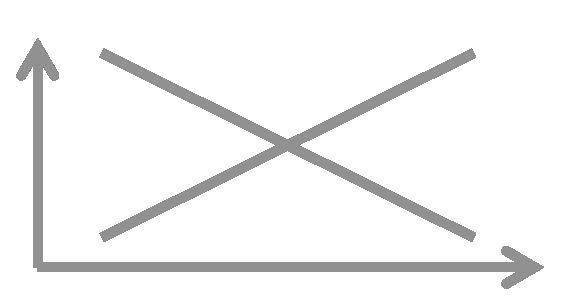
\includegraphics[width = .95\columnwidth]{figures/placeholder}
  \caption{.}
  \label{f:tpcc} 
  \end{subfigure}
  \begin{subfigure}[t]{.48\columnwidth}
  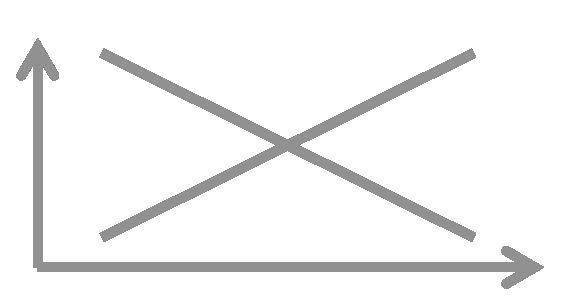
\includegraphics[width = .95\columnwidth]{figures/placeholder}
  \caption{.}
  \label{f:auctionmark} 
  \end{subfigure}
  \caption{Benchmark Performance}

\end{figure}

\subsection{Synthetic data}
The factors influence the complexity of the MILP-based approach fall 
into four aspects: skewness, $s$; log size, $N_q$; database size $N_D$; and 
query complexity $N_w$. In this section, we focus on 
evaluate the proposed algorithm(s)
by adjusting these four factors. 
\subsubsection{Skew}
We generate query log at 4 different skewness levels from uniform to 
super skewed with $s = 0, 1e-7, 0.5, 1$. As we can see as query log
is more skewed, the execution time for solving same amount of queries 
increase. This is also due to the fact that increasing skewness also
increase the query dependency, which, in turn, increase the searching
space in the MILP problem.
 
 \begin{figure}[h]
\centering
  \begin{subfigure}[t]{.48\columnwidth}
  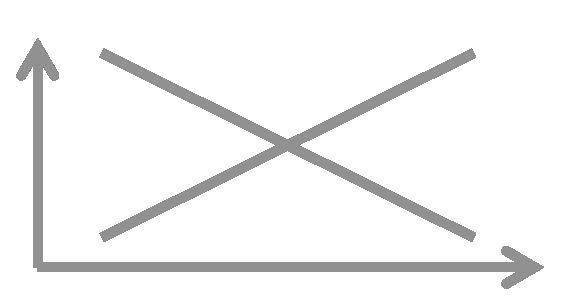
\includegraphics[width = .95\columnwidth]{figures/placeholder}
  \caption{.}
  \label{f:multiquery} 
  \end{subfigure}
  \caption{Log size. }
\end{figure}

\subsubsection{Scalabality: log size}
 \begin{figure}[h]
\centering
  \begin{subfigure}[t]{.48\columnwidth}
  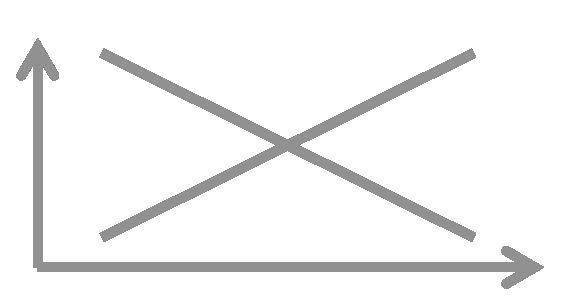
\includegraphics[width = .95\columnwidth]{figures/placeholder}
  \caption{.}
  \label{f:multiquery} 
  \end{subfigure}
  \caption{MILP-based Approach and Extensions on Multi-Query. }
\end{figure}

\subsubsection{Scalability: database size}
We adjust the initial database sizes from 100 to 100,000 and 
while maintain the same range $r$ in each query. As we can see, 
for the same corrupt query index, the MILP-based approaches require
similar amount of time to derive the log repair. 

 \begin{figure}[h]
\centering
  \begin{subfigure}[t]{.48\columnwidth}
  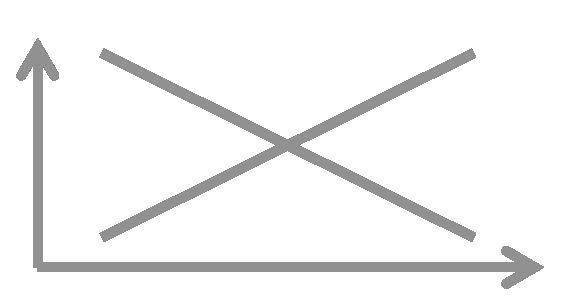
\includegraphics[width = .95\columnwidth]{figures/placeholder}
  \caption{.}
  \label{f:multiquery} 
  \end{subfigure}
  \caption{Database size}
\end{figure}


\subsubsection{Scalability: query complexity}
In the end, we evaluate the MILP-based approaches by adjust 
the query complexity: number of predicates, $N_w$, in the 
update query while maintain the range $r$ the same. 

 \begin{figure}[h]
\centering
  \begin{subfigure}[t]{.48\columnwidth}
  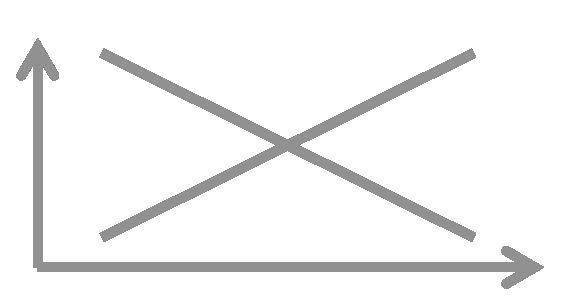
\includegraphics[width = .95\columnwidth]{figures/placeholder}
  \caption{.}
  \label{f:multiquery} 
  \end{subfigure}
  \caption{Query complexity }
\end{figure}

}
\subsubsection{Handling Noise}

In this set of experiments, we add false negative complaints to the input
complaint set and evaluate our noise handling algorithms (Section~\ref{sec:noise}).
To generate false negatives ($FN$), we select a random subset of the true complaint set.


\begin{figure}[h]
\centering
  \begin{subfigure}[t]{.48\columnwidth}
  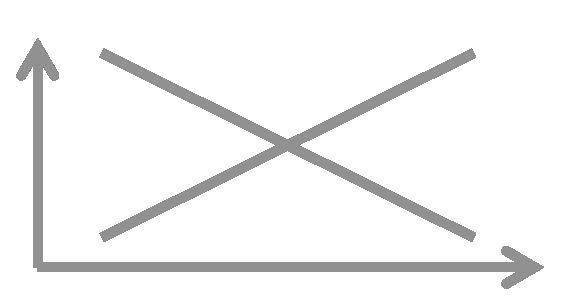
\includegraphics[width = .95\columnwidth]{figures/placeholder}
  \caption{.}
  \label{f:falsenegative} 
  \end{subfigure}
  \caption{cap}

\end{figure}


Figure~\ref{f:falsenegative} varies $FN \in \{\}$.














\iffalse
\subsubsection{Algorithms}

\sys fixes query logs in two distinct steps: first, we filter the query log using 
provenance information and roll back the queries to compute the $ideal$ states of the database.
Second, we apply the solver algorithms (Section~\ref{}) to speculatively fix the query.

We consider the roll-back algorithm in batches of $n_{rollback}$.

\begin{itemize}
\item Combined:  combine rollback and query fixing in a single CPLEX problem
\item $R_n-CPLEX$: 
\item DT
\item Box,Density
\end{itemize}



\subsubsection{Comparison}

\begin{itemize}
\item Query By Example algorithm
\item Quoc's ConQueR
\end{itemize}

Conditions, given a database ${\cal D}$ and query log $qlog$:

\begin{itemize}
\item {\bf $N_\mathcal{D}$: } Size of the database (number of tuples)
\item {\bf $N_{dim}$:} Dimensionality of the database.
\item {\bf $N_\mathcal{Q}$:} Vary number of queries in $qlog$.
\item {\bf $N_{pred}$:} The number of predicates in each UPDATE query's WHERE condition.
\item {\bf $N_{ins}$: } When corrupting the log, the number of values in INSERT to corrupt.
\item {\bf $N_{set}$: } When corrupting the log, the number of clauses in SET that are corrupted.
\item {\bf $N_{where}$: } When corrupting the log, the number of attributes in the WHERE clause that are corrupted.
\item {\bf $idx \in [0, 1]$: } The index of the query in the query log that was corrupted as a percentage of the query log.  
      For example $Idx = 0.0$ is the oldest query in the log, whereas $Idx = 1.0$ is the most recent query position.
\item {\bf $p_{I}$: } Percentage of INSERT queries in the query log (as compared to UPDATEs).
\item {\bf $p_{pk}$: } Percentage of UPDATE queries with primary key filter clauses as compared to range clauses over non-primary key attributes.
\item {\bf $p_{FP}$: } Percentage of false positives in the complaint set.
\item {\bf $p_{FN}$: } Percentage of false negatives in the complaint set.
\end{itemize}



\subsection{Exact Experiments}

\begin{itemize}
\item $N_\mathcal{D} \in \{10, 100, 1000\}$
\item $N_q \in \{10, 20, 50, 100\}$
\item $N_{dim} = 4$
\item $N_{pred} \in \{1, 2, 3\}$
\item $N_{where} = \{1, 2\}$
\item $Idx = \{0, 0.5, 1\}$
\end{itemize}

\subsection{Rollback and \qfix Microexperiments}


The first set of experiments seeks to understand the effectiveness of the database rollback
algorithm.  We use a synthetic dataset (\ewu{describe}) and execute the rollback algorithm
while varying the query batch size.

\subsection{End-to-end experiments}

\subsubsection{Complete Complaint Set}

\subsubsection{Complaint Set with Noise}

\begin{itemize}
\item $N_\mathcal{D} \in \{10, 100, 1000\}$
\item $N_q \in \{10, 20, 50, 100\}$
\item $N_{dim} = 4$
\item $N_{pred} \in \{1, 2, 3\}$
\item $N_{attrs} = \{1, 2\}$
\item $Idx = \{0, 0.5, 1\}$
\end{itemize}

\subsection{TPC-C Experiment}


\deprecate{
  \subsection{Single-Query Log}

  In the first set of experiments, we evaluate the simplest case where there
  is a single update query.  In each experiment, we vary the DBSize,
  NClauses, as well as the number of clauses in the query that have
  been corrupted and report the metrics described above.  We first 
  compare the learning algorithms on a complete complaint set, then evaluate them
  using incomplete complaint sets with varying percentages of false positive and negative complaints.

  \subsubsection{Complete Complaints}

  {\it Vary DBSize

  Vary NClauses, corrupt 1 and 2 clauses
  }

  We found that CPLEX and BBOX identify the correct fix, however their
  running times are significantly higher than DTree.  This is because
  CPLEX is an exact solution, as compared to DTree, whose poor early
  splitting decisions can adversely affect the final tree structure.

  \subsubsection{Incomplete Complaints}


  {\it 
  Vary DBSize

  Vary NClauses, corrupt 1 and 2 clauses

  Each line is plots has different perc FP
  }

  We first increased the number of false positives in the complaint set (no false negatives).
  Figure~\ref{f:single_incomplete_fp} shows how the fix quality and running time vary as the
  percentage of false positives increases.   Compared variations of CPlex and Bounding box with varying
  density thresholds (?).

  Each line varies perc FN

  We then varied the number of false negatives while keeping the percentage of false positives fixed at 5\%.
  Figure~\ref{f:single_incomplete_fn} 


  \subsection{Increased Query Log Size}

  In the following set of experiments, we increase the number of
  queries in the log while varying ?.  The number of corrupted queries
  is still one.  In these experiments, we set the DBSize to 10000,
  the default NClauses to 4, and the number of corrupted clauses to
  2.   We first show results for varying the false positives and
  negatives in the complaint set and comparing the algorithms described
  in Section~\ref{s:incomplete-algs}.  We then evaluate the efficacy
  of of provenance-based query log filtering, which reduces the running
  time without affecting the result quality.

  To generate the false-positives, we randomly sample without replacement
  from the tuples in the database that are not in the true complaint
  set.

  \subsection{False Positive}

  Vary false positives (1 graph)


  \subsection{False Negative}

  Vary false negatives (1 graph)

  \subsubsection{Filtering Queries}

  We also compared the provenance-based filtering techniques in the above experiments
  to measure their effectiveness at reducing the running time.  We varied the complexity of the update 
  WHERE clauses to control the amount that queries in the log overlap in their updates.  The query log contained 50 update WHERE queries.
  The quality of the suggested fixes were the same,  As the clauses became less complex, the likelihood 
  of overlap increased, and increased the amount of queries that affected the complaint sets.


  \begin{figure}[h]
  \centering
  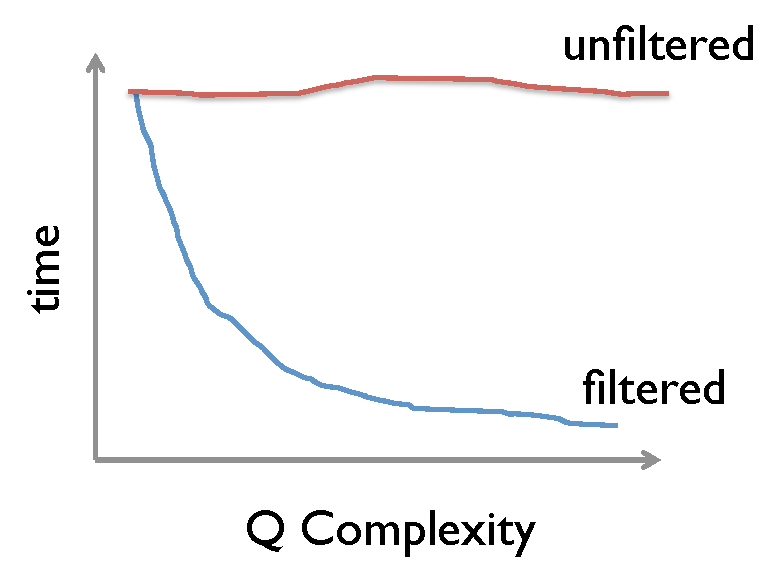
\includegraphics[width = 2in]{figures/complete_qfilter_complexity}
  \caption{Varying query complexity.}
  \label{f:complete_qfilter_complexity} 
  \end{figure}



  \subsection{Multi-Query}

  Using a previous experimental configuration, we varied the number of queries that are corrupted.  Figures~\ref{}
  show the quality and running times of the results for a query log of size 1000 and dbsize of 100k.  
  As we can see, the cost increases quadratically with each corrupted query and the accuracy of the proposed fixes increases marginally.  
  This is because XXX.

  We focus on two scenarios.  {\bf Try multiple corruptions that don't overlap (provenance-wise) with each other}.  This is the condition of multiple silo'd that
  corrupt their own logs.  Then {\bf Try multiple corrupted queries where one query modifies the updated state of the other}.  This shows that
  it is really hard and hopefully we get close?



  To better understand the algorithm, we plot the quality metrics after each fixed query and measure how quickly \sys converges to the final result. 
  This suggests that an incremental approach where the user can set a threshold to stop the algorithm may be effective.



  \subsection{Real Transactional Workload}

  We used the web application workload, and evaluated our alogirthms with artifically injected corruptions.
  We compared two types of corruptinos.  In figure~\ref{f:real_existing}, we randomly picked a single existing 
  query and corrupted its value.  If the query was an INSERT, we randomly pick a value and perturbed it.
  If the transaction was an UPDAET, we randomly varied the SET or WHERE clauses.   We re-ran this
  100 times and plot the average and standard deviation of the results.

}
\fi
